\documentclass{article}
\usepackage{graphicx}
\usepackage[top=1.00in,
	bottom=1.00in,
	left=0.75in,
	right=0.75in]{geometry}
\usepackage[colorlinks=true,
	citecolor=black,
	linkcolor=blue,
	urlcolor=black,
	breaklinks=true]{hyperref}
\begin{document}

\section*{Introduction}

\noindent Once upon a time, there was prior work \cite{Ernst1987,Kuehn2008feb}. 

Next consider math.  Inline math is nice, $\alpha = 2$, as are stand-alone equations,
\begin{equation}
\int_0^{\infty} e^{-x} dx = 1.
\end{equation}

Finally, a figure.  See Fig.~\ref{fig:sine} below.

\bibliographystyle{bst/grants-CV}
\bibliography{bib/jam99.bib}

\newpage

\begin{figure}
\centering
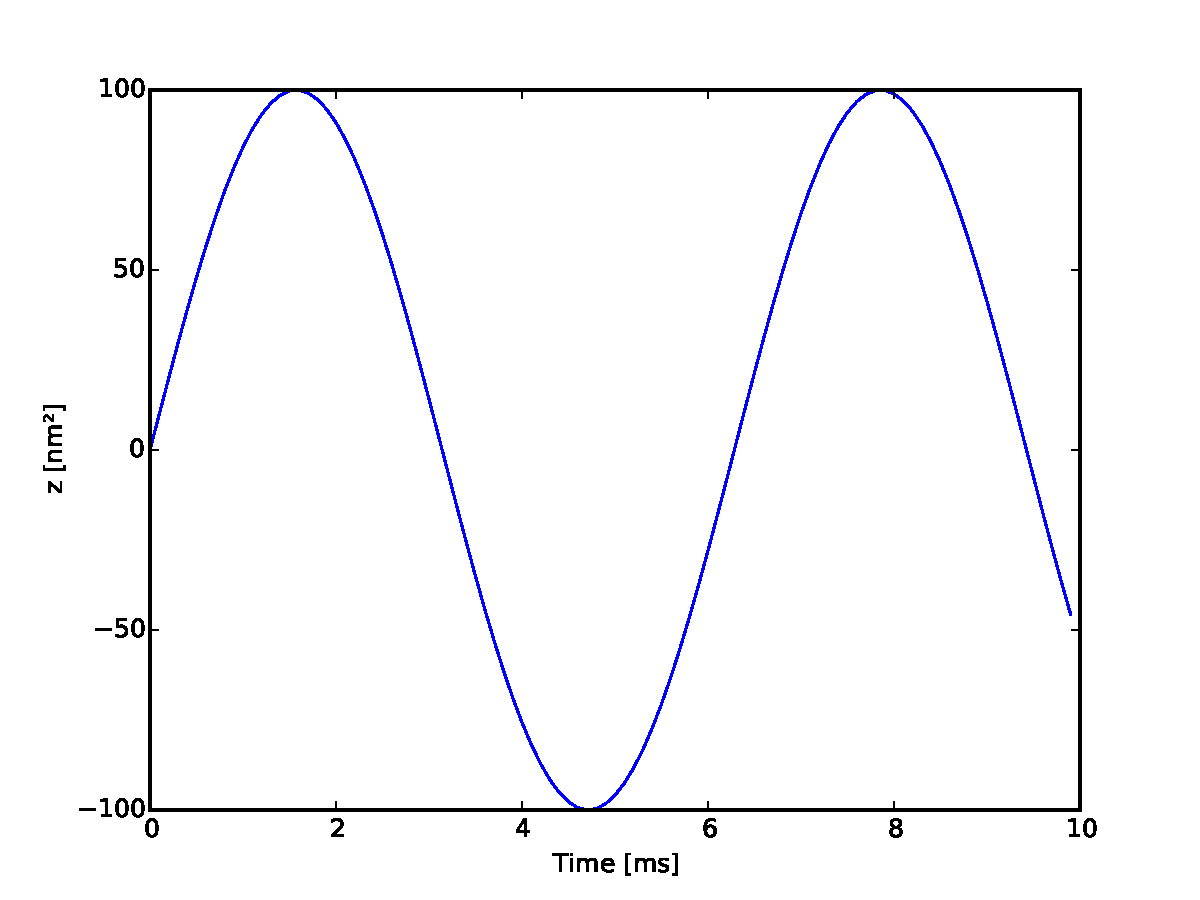
\includegraphics[width=6.50in]{figs/ex.pdf}
\caption{This is a figure.}
\label{fig:sine}
\end{figure}

\end{document}